\section{Hypothèse de pertinence}
\label{section:4.4-HYPOTHESE-PERTINENCE}

	%%% Introduction / Transition.
	Jusqu'à présent, nous avons analysé la performance et l'évolution des résultats de notre implémentation du \textit{clustering} interactif à l'aide d'une vérité terrain (cf. calcul de \texttt{v-measure}).
	Cependant, une telle référence n'est pas accessible en situation réelle (l'objectif de notre méthode est précisément de la construire).
	Nous devons donc nous intéresser à d'autres moyens d'estimer la pertinence des bases d'apprentissages obtenus et de définir comment définir l'exploitabilité d'un résultat.
	Ainsi, nous aimerions vérifier l'hypothèse suivante :
	
	%%% Formulation des hypothèses:
	\begin{tcolorbox}[
		title=\faVial~\textbf{Hypothèse de pertinence}~\faVial,
		colback=colorTcolorboxHypothesis!15,
		colframe=colorTcolorboxHypothesis!75,
		width=\linewidth
	]
		« \textbf{
			Au cours d'une méthodologie d'annotation basée sur le \textit{clustering} interactif, il est possible à un expert métier d'évaluer rapidement la pertinence de la base d'apprentissage en construction sans utiliser de vérité terrain.
		} » \\
		
		% Figure.
		La figure~\ref{figure:4.4-HYPOTHESE-PERTINENCE} illustre cette hypothèse et l'espoir de pouvoir caractériser la qualité de la base d'apprentissage en cours de construction en fonction d'une valeur métier exprimée par un expert.
		%
		\begin{figure}[H]  % keep [H] to be in the tcolorbox.
			\centering
			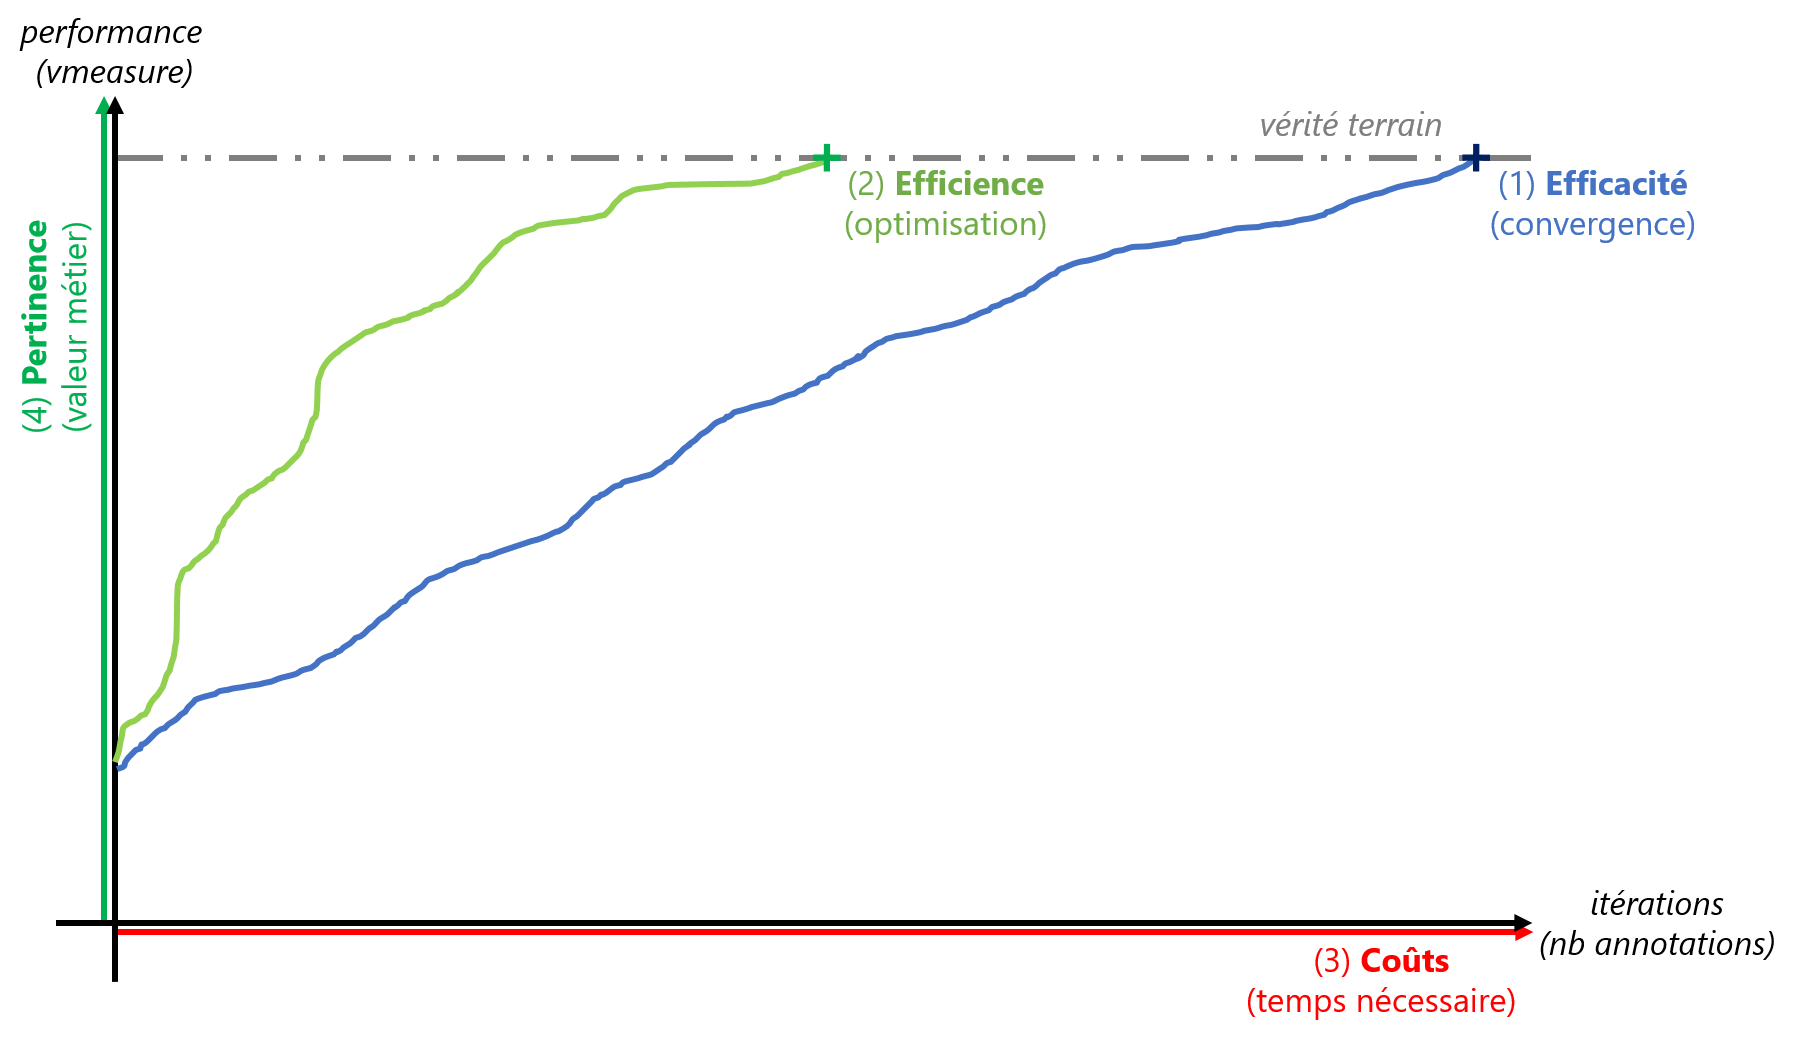
\includegraphics[width=0.95\textwidth]{figures/hypotheses-04-pertinence}
			\caption{Illustration des études réalisées sur le \textit{clustering} interactif (\textit{étape 4/6}) en schématisant l'évolution de la pertinence (\textit{valeur métier évaluée par l'expert et exprimé en nombre de clusters}) d'une base d'apprentissage en cours de construction en fonction du coût temporel de la méthode (\textit{temps nécessaire à l'expert métier et à la machine}).}
			\label{figure:4.4-HYPOTHESE-PERTINENCE}
		\end{figure}

	\end{tcolorbox}
		
	% Résumé de l'étude.
	Afin de vérifier cette hypothèse, nous explorons trois approches :
	\begin{itemize}
		\item une \textbf{vérification par un expert} du partitionnement des données obtenus, en parcourant manuellement le contenu des \textit{clusters} et en donnant un avis sur l'exploitabilité de ces derniers (cf. sous-section~\ref{section:4.4.1-ETUDE-PERTINENCE-VERIFICATION-MANUELLE}) ;
		\item une analyse des \textbf{patterns linguistiques saillants} dans la base d'apprentissage à l'aide d'une stratégie de sélection des composantes principales d'un modèle (cf. sous-section~\ref{section:4.4.2-ETUDE-PERTINENCE-PATTERNS-LINGUISTIQUES}),
		\item et une approche utilisant un \textbf{résumé automatique de thématique} par un modèle de langue, permettant de décrire succinctement le contenu des \textit{clusters} en une phrase. (cf. sous-section~\ref{section:4.4.3-ETUDE-PERTINENCE-RESUME-AUTOMATIQUE}).
	\end{itemize}
	
	
	%%%
	%%% Subsection 4.4.1: Étude d'une vérification manuelle de la valeur métier d'une base d'apprentissage par un expert
	%%%
	\subsection{Étude d'une vérification manuelle de la valeur métier d'une base d'apprentissage par un expert}
	\label{section:4.4.1-ETUDE-PERTINENCE-VERIFICATION-MANUELLE}
		
		% Objectif de l'expérience.
		\todo[inline]{A REDIGER: objectif de l'expérience}
		Afin d'estimer la pertinence d'un résultat de \textit{clustering}, notre première intuition consiste à demander l'avis d'un expert sur la base d'apprentissage en cours de construction.
	
		%%% Protocole expérimental.
		\subsubsection{Protocole expérimental}
			\todo[inline]{A REDIGER}
			
			% Axiome.
			\begin{leftBarWarning}
				Par manque de personnes compétentes sur le jeu de données utilisé, les annotations réalisées dans cette étude n'ont pu être faites que par un seul annotateur.
				Afin de limiter les biais pouvant surgir à cause de cette contraintes, nous avons reproduit plusieurs fois l'analyse sur des \textit{clusters} différents et nous discutons de la moyenne des résultats obtenus.
			\end{leftBarWarning}
			
			% Pseudo-code.
			Pour résumer le protocole expérimental adapté, vous pouvez vous référer au pseudo-code décrit dans Alg.~\ref{algorithm:4.4.1-ETUDE-PERTINENCE-VERIFICATION-MANUELLE}.
			%
			\begin{algorithm}[!htb]
				\begin{algorithmic}[1]
					\Require jeux de données annotés (vérité terrain) de tailles différentes
					\State \textbf{initialisation (données)}: récupérer ou générer les données et la vérité terrain
					\State \textbf{initialisation (contraintes)}: créer une liste vide de contraintes
					\State \textbf{prétraitement}: supprimer le bruit dans les données avec \texttt{prep.simple}
					\State \textbf{vectorisation}: transformer les données en vecteurs avec \texttt{vect.tfidf}
					\State \textbf{clustering initial}: regrouper les données par similarité avec \texttt{clust.kmeans.cop}
					\State \textbf{évaluation manuelle}: juger de l'exploitabilité de chaque \textit{cluster}
					\Repeat
						\State \textbf{échantillonnage}: sélectionner de nouvelles contraintes à annoter
						\State \textbf{simulation d'annotation}: ajouter des contraintes avec \texttt{samp.closest.diff}
						\State \textbf{clustering}: regrouper les données par similarité avec \texttt{clust.kmeans.cop}
						\State \textbf{évaluation manuelle}: juger de l'exploitabilité de chaque \textit{cluster}
						\State \textbf{labellisation manuelle}: nommer chaque \textit{cluster} exploitable
					\Until{annotation de toutes les contraintes possibles}
					\State \textbf{analyse}: afficher l'évolution de l'exploitabilité de chaque itération de \textit{clustering}
					\Ensure discussion sur la complexité de la tâche et sur l'évolution de l'exploitabilité
				\end{algorithmic}
				\caption{Description en pseudo-code du protocole expérimental de l'étude de vérification manuelle de la valeur métier d'une base d'apprentissage.}
				\label{algorithm:4.4.1-ETUDE-PERTINENCE-VERIFICATION-MANUELLE}
			\end{algorithm}
				
			
			% Détails de l'expérience.
			
			
			% Référence scripts.
			\begin{leftBarInformation}
				Les scripts de l'expérience, réalisés avec des \textit{notebooks} Python (\cite{van-rossum-drake:2009:python-reference-manual}), sont disponibles dans un dossier dédié de~\cite{schild:2021:cognitivefactory-interactiveclusteringcomparativestudy}.
			\end{leftBarInformation}
			

		%%% Résultats
		\subsubsection{Résultats obtenus}
			\todo[inline]{A REDIGER}
		
			% Description statistiques.
			\todo[inline]{A REDIGER: On peut voir 3 phases: INEXPLOITABLE / DE PLUS EN PLUS EXPLOITABLE / EXPLOITABLE ; les partiellement exploitables servent de transition.}
			
			% Exemple.
			\todo[inline]{A REDIGER: tableau avec exemples ?}
			
			% Figure.
			%
			\begin{figure}[!htb]
				\centering
				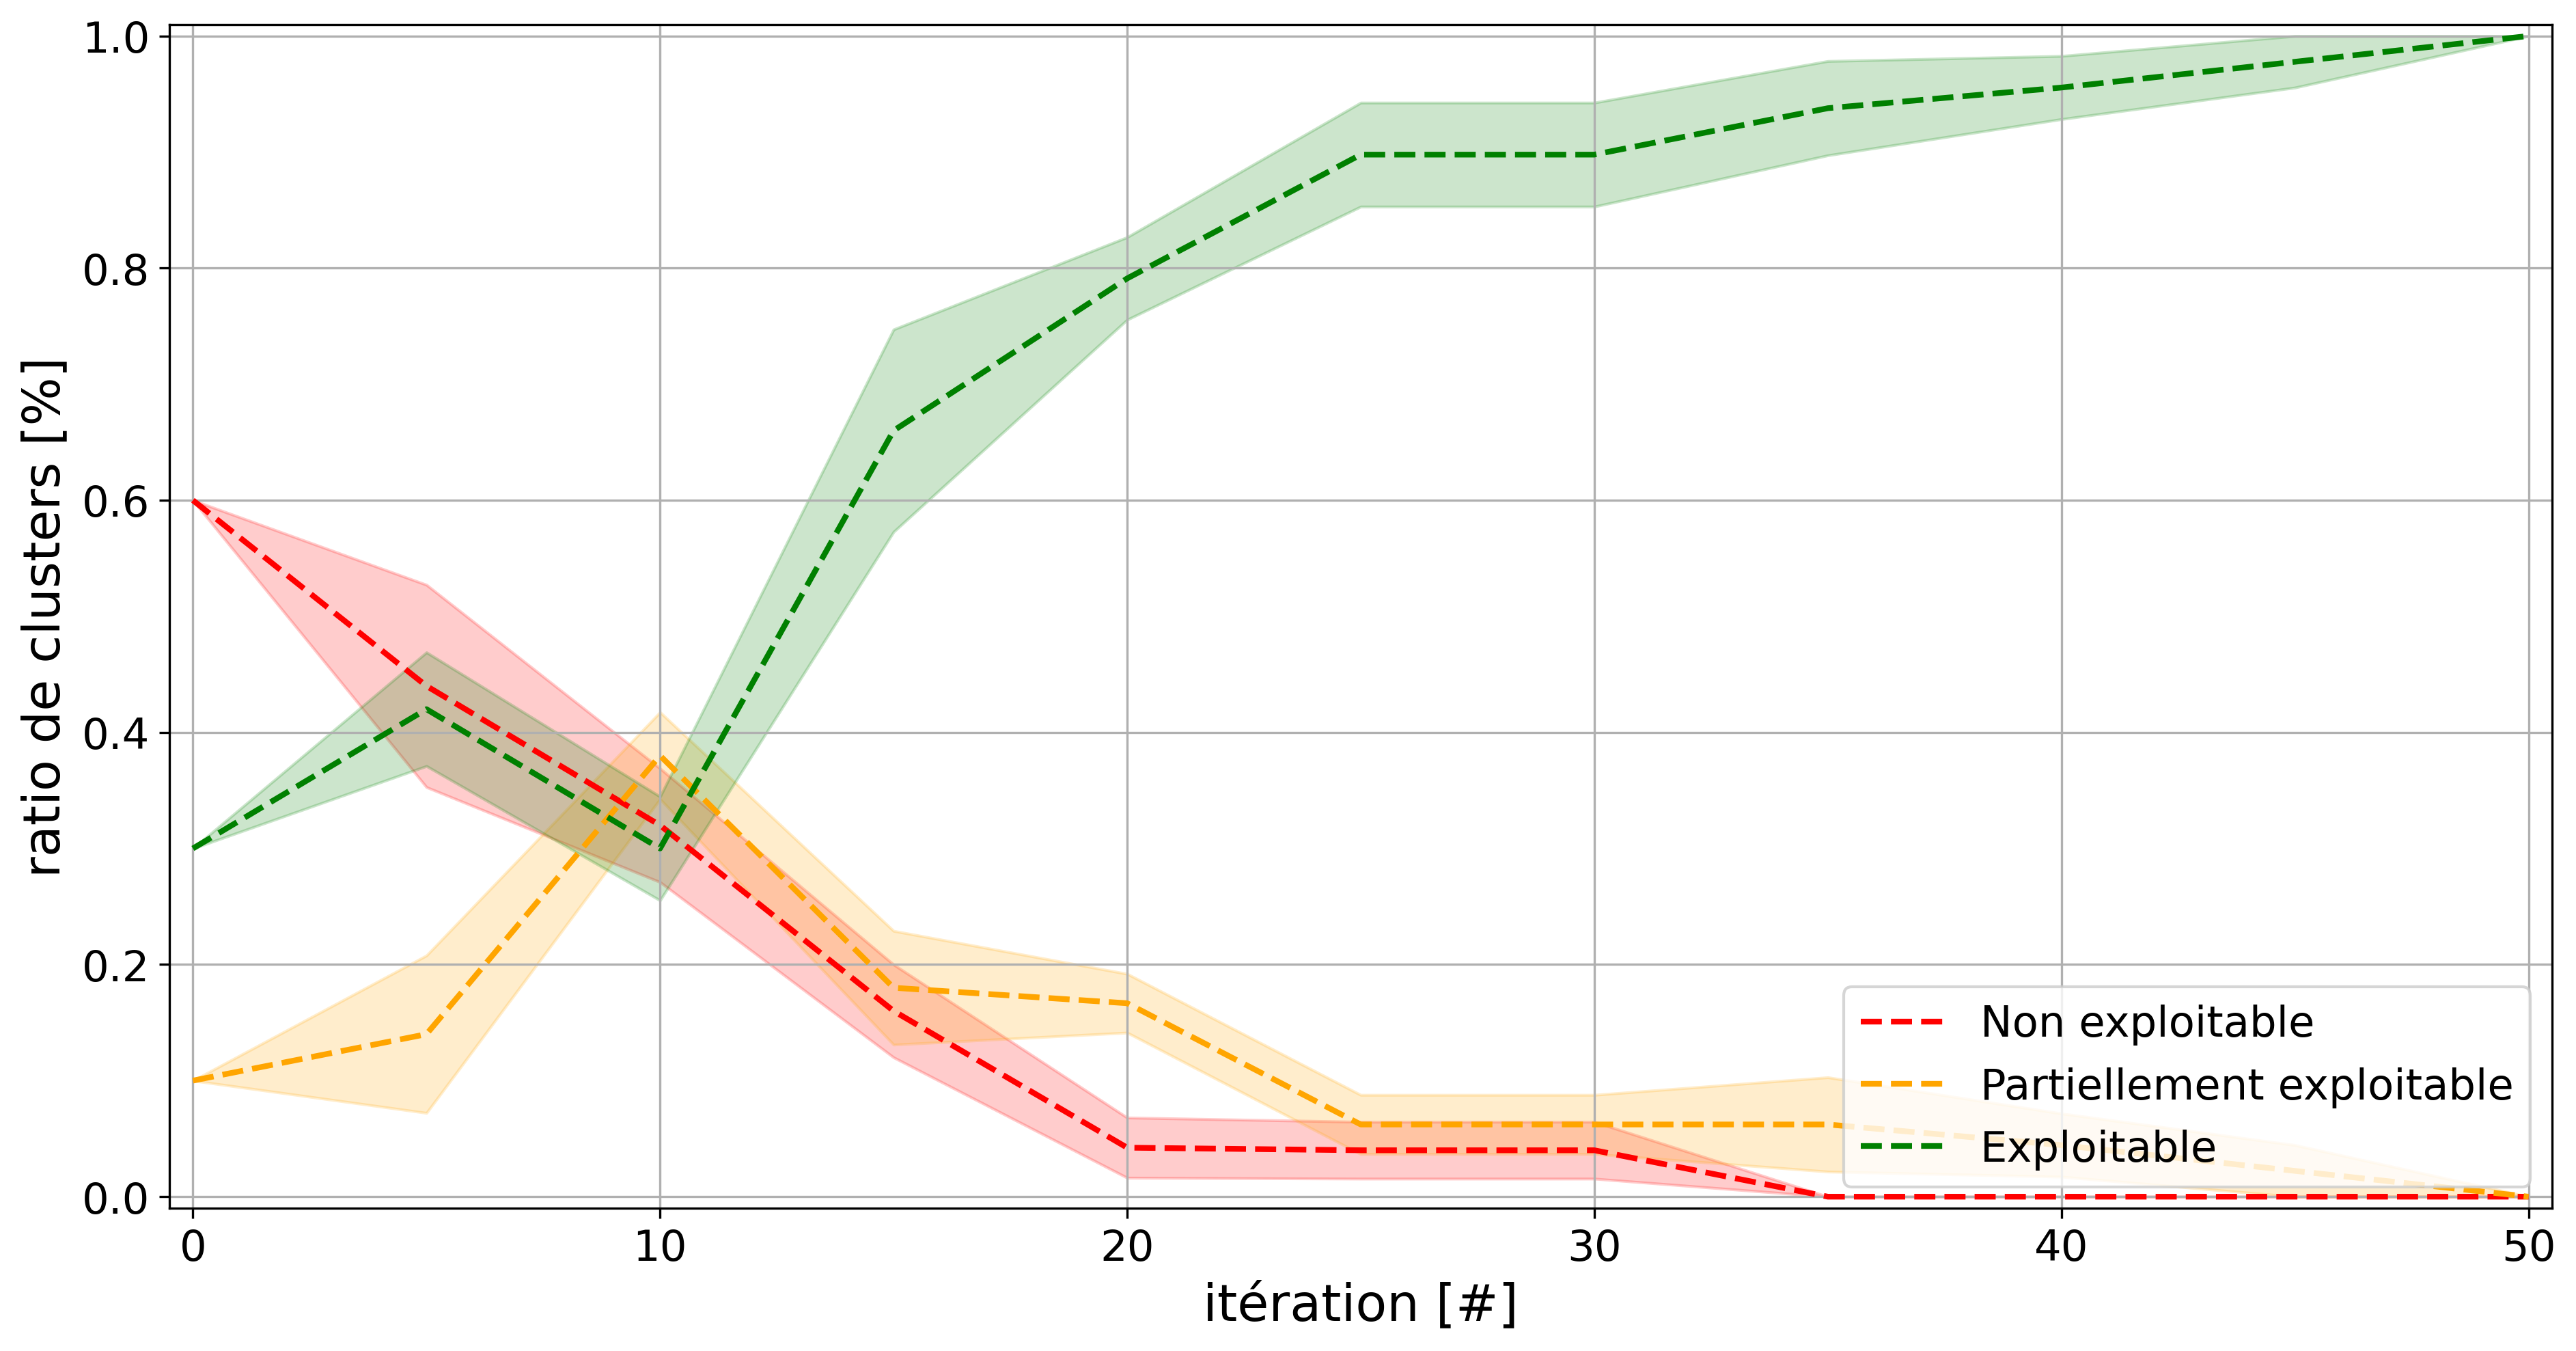
\includegraphics[width=0.95\textwidth]{figures/etude-pertinence-llm-check-clustering-annotation-favori}
				\caption{Évolution de la pertinence métier moyenne d'un résultat en fonction du nombre d'itérations de la méthode.
				La pertinence est estimée manuellement en trois niveaux (\texttt{non exploitable}, \texttt{partiellement exploitable} et \texttt{exploitable}) sur la base du contenu des \textit{clusters} et est exprimée en proportion du nombre de \textit{clusters} concernés.}
				\label{figure:4.4.1-ETUDE-PERTINENCE-VERIFICATION-MANUELLE}
			\end{figure}

		%%% Discussion
		\subsubsection{Discussion}
			\todo[inline]{A REDIGER}
		
			% Remaques expérience utilisateur.
			\todo[inline]{A REDIGER: C'est super fastidieux, sensible à l’inattention, ...}
			
			% Conclusions et suggestion.
	
	
	%%%
	%%% Subsection 4.4.2: Etude des patterns linguistiques pertinents à l'aide de la \textit{Features Maximization}
	%%%
	\subsection{Étude des patterns linguistiques pertinents à l'aide de la \textit{Features Maximization}}
	\label{section:4.4.2-ETUDE-PERTINENCE-PATTERNS-LINGUISTIQUES}
		
		% Objectif de l'expérience.
		\todo[inline]{A REDIGER: objectif de l'expérience}
	
		%%% Protocole expérimental.
		\subsubsection{Protocole expérimental}
			\todo[inline]{A REDIGER}
			% Axiome.
			% Pseudo-code.
			% Détails de l'expérience.
			
			% Référence scripts.
			\begin{leftBarInformation}
				Les scripts de l'expérience, réalisés avec des \textit{notebooks} Python (\cite{van-rossum-drake:2009:python-reference-manual}), sont disponibles dans un dossier dédié de~\cite{schild:2021:cognitivefactory-interactiveclusteringcomparativestudy}.
				L'implémentation de la maximisation des traits est accessible ici dans~\cite{schild:2023:cognitivefactory-featuresmaximizationmetric}.
			\end{leftBarInformation}

		%%% Résultats
		\subsubsection{Résultats obtenus}
			\todo[inline]{A REDIGER}
		
			% Description statistiques.
			
			% Exemple.
			\todo[inline]{A REDIGER: tableau avec exemples ?}

		%%% Discussion
		\subsubsection{Discussion}
			\todo[inline]{A REDIGER}
		
			% Remaques expérience utilisateur.
			\todo[inline]{A REDIGER: C'est pas adapté pour un expert métier, mais ça peut être utilisé pour de l'affichage}
			
			% Exemple.
			\todo[inline]{A REDIGER: tableau avec exemples ?}
			
			% Conclusions et suggestion.
	
	
	
	%%%
	%%% Subsection 4.4.3: Etude d'un résumé automatique des \textit{clusters} à l'aide d'un modèle de langue.
	%%%
	\subsection{Étude d'un résumé automatique des \textit{clusters} à l'aide d'un modèle de langue}
	\label{section:4.4.3-ETUDE-PERTINENCE-RESUME-AUTOMATIQUE}
		
		% Objectif de l'expérience.
		\todo[inline]{A REDIGER: objectif de l'expérience}
	
		%%% Protocole expérimental.
		\subsubsection{Protocole expérimental}
			\todo[inline]{A REDIGER}
			% Axiome.
			% Pseudo-code.
			% Détails de l'expérience.
			
			% Référence scripts.
			\begin{leftBarInformation}
				Les scripts de l'expérience, réalisés avec des \textit{notebooks} Python (\cite{van-rossum-drake:2009:python-reference-manual}), sont disponibles dans un dossier dédié de~\cite{schild:2021:cognitivefactory-interactiveclusteringcomparativestudy}.
				L'appel à un modèle de langue se fait grâce à la librairie \texttt{openai}.
			\end{leftBarInformation}

		%%% Résultats
		\subsubsection{Résultats obtenus}
			\todo[inline]{A REDIGER}
		
			% Description statistiques.
			\todo[inline]{A REDIGER: On peut voir 3 phases: INEXPLOITABLE / DE PLUS EN PLUS EXPLOITABLE / EXPLOITABLE ; les partiellement exploitables sont pas très présents.}
			
			% Exemple.
			\todo[inline]{A REDIGER: tableau avec exemples ?}
			
			% Figure.
			%
			\begin{figure}[!htb]
				\centering
				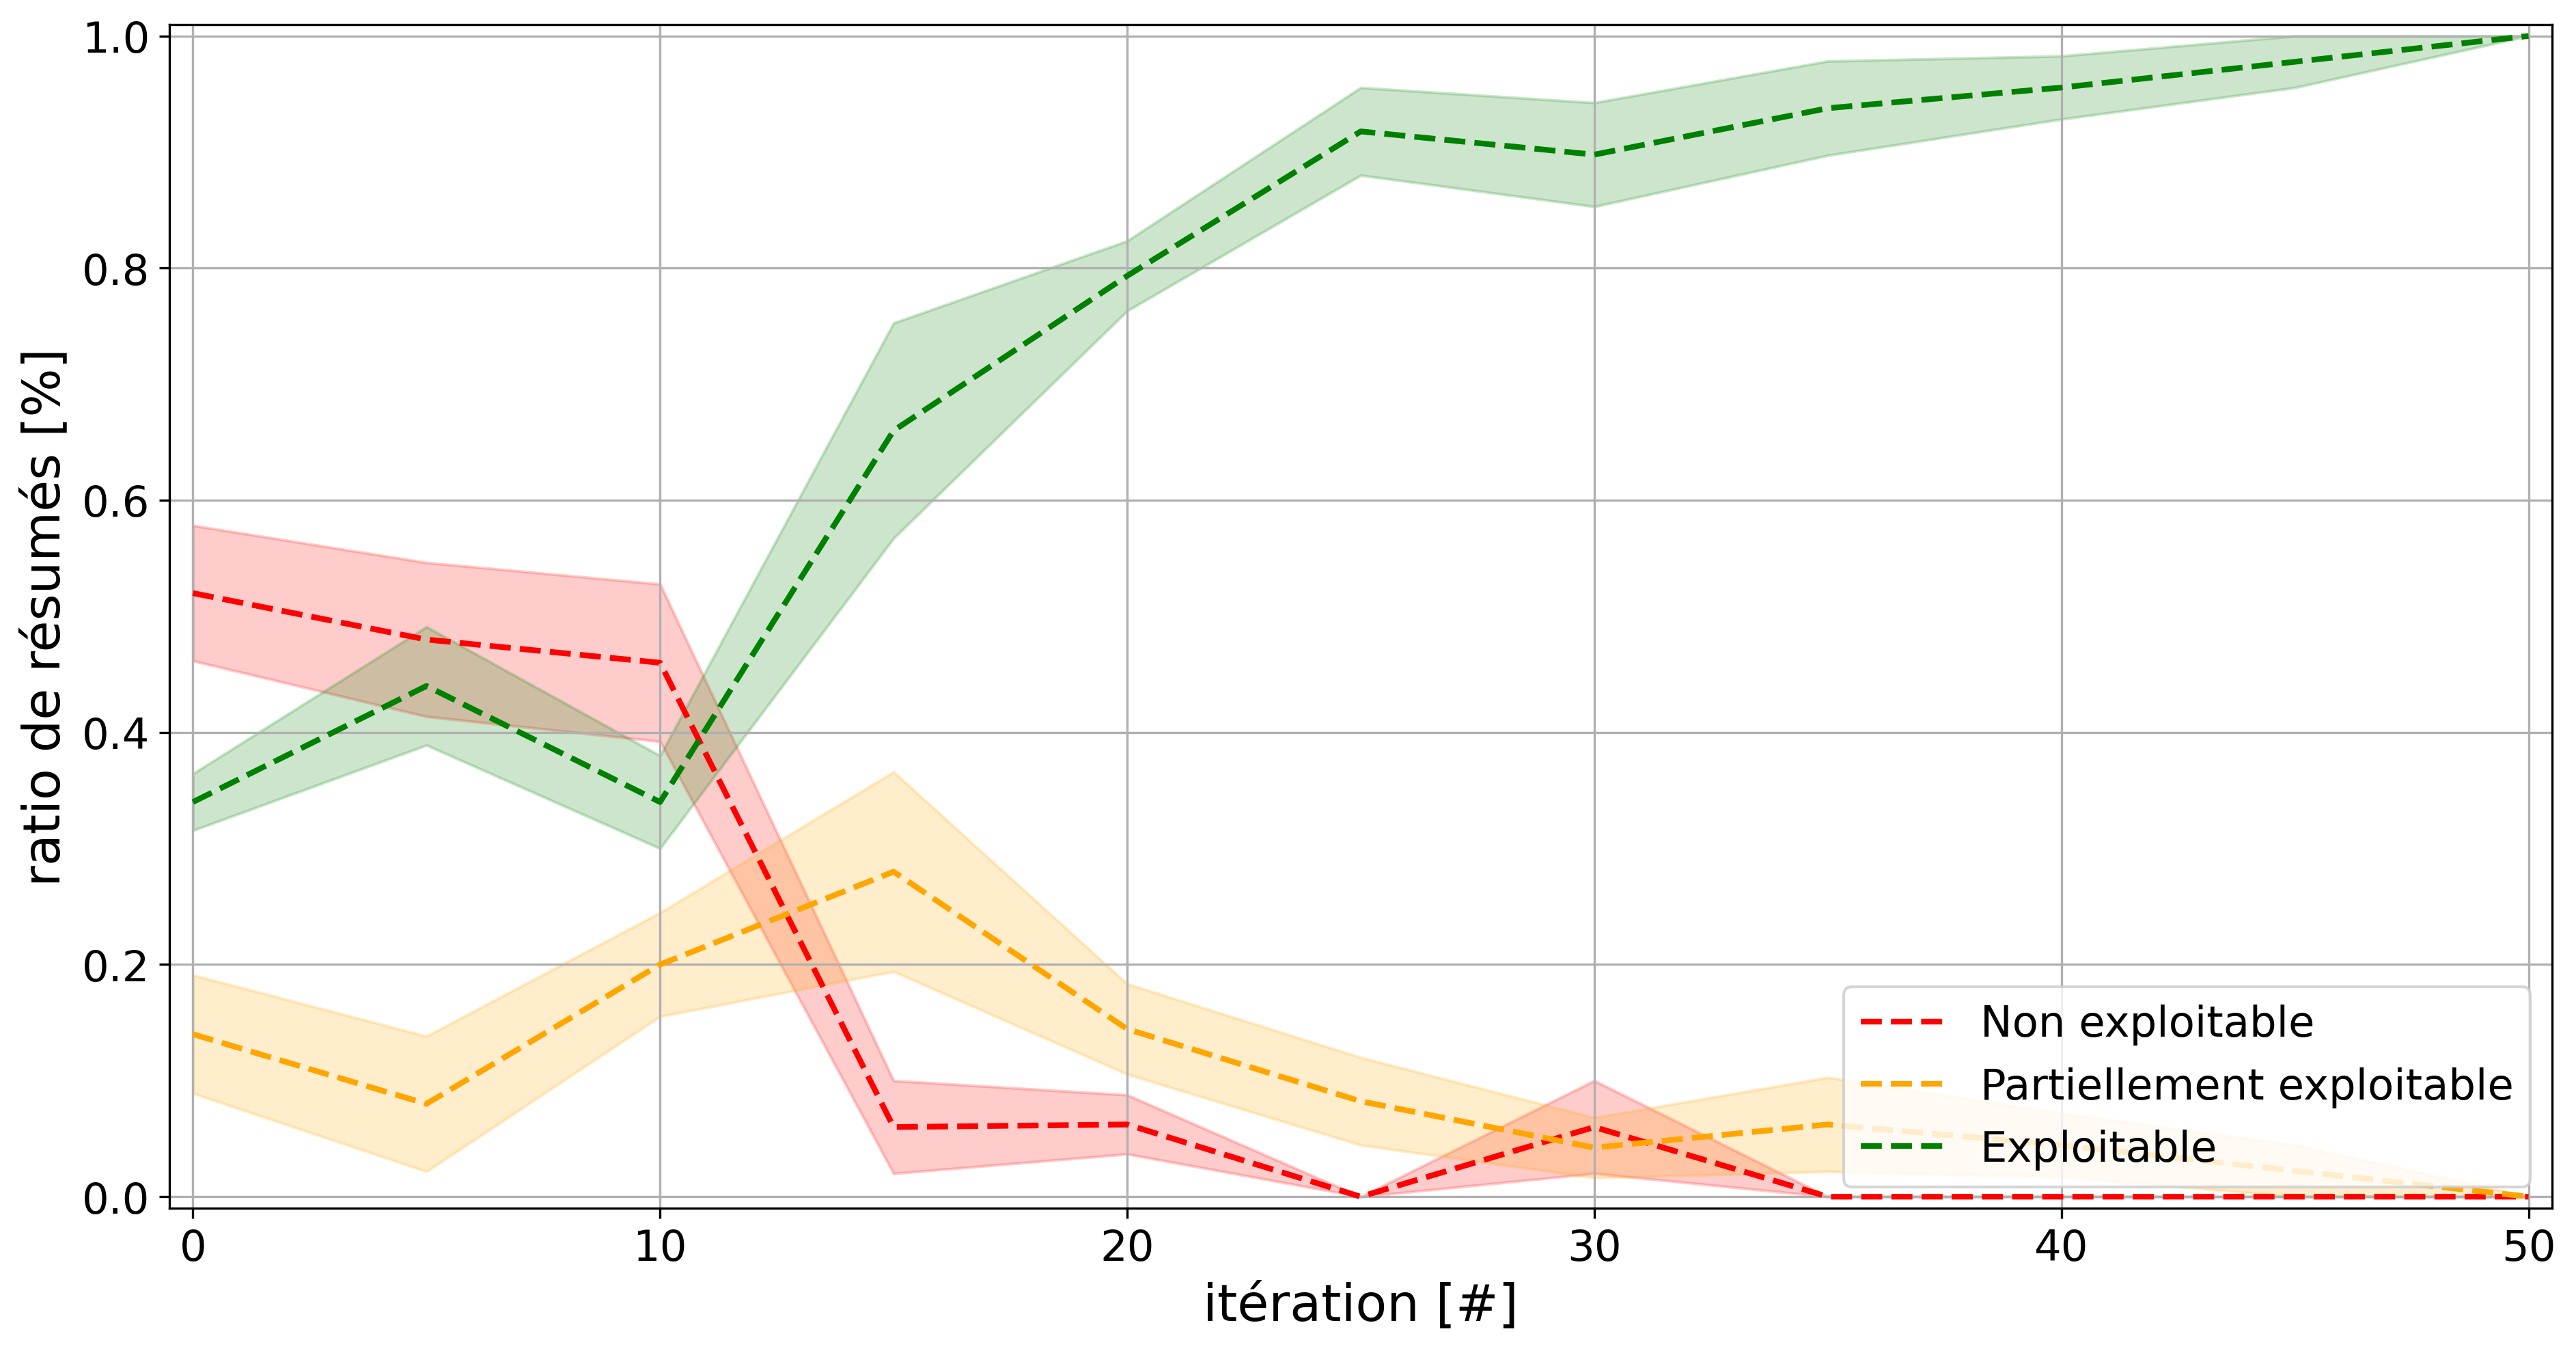
\includegraphics[width=0.95\textwidth]{figures/etude-pertinence-llm-check-resume-annotation-favori}
				\caption{Évolution de la pertinence métier moyenne d'un résultat en fonction du nombre d'itérations de la méthode.
				La pertinence est estimée en trois niveaux (\texttt{non exploitable}, \texttt{partiellement exploitable} et \texttt{exploitable}) sur la base du résumé automatique des \textit{clusters} par un modèle de langue et est exprimée en proportion du nombre de \textit{résumés} concernés.}
				\label{figure:4.4.3-ETUDE-PERTINENCE-RESUME-AUTOMATIQUE}
			\end{figure}

		%%% Discussion
		\subsubsection{Discussion}
			\todo[inline]{A REDIGER}
		
			% Remaques expérience utilisateur.
			\todo[inline]{A REDIGER: C'est super pratique, super accessible}
			\todo[inline]{A REDIGER: C'est parfois un peu ambigu...}
			
			% Conclusions et suggestion.
	
	
	%%%
	%%% Subsection 4.4.4: Étude de la cohérence statistique de la base d'apprentissage en cours de construction
	%%%
	%\subsection{Étude de la cohérence statistique de la base d'apprentissage en cours de construction}
	%\label{section:4.4.4-ETUDE-PERTINENCE-COHERENCE}
	%	
	%	% Objectif de l'expérience.
	%	\todo[inline]{A REDIGER: objectif de l'expérience}
	%
	%	%%% Protocole expérimental.
	%	\subsubsection{Protocole expérimental}
	%		\todo[inline]{A REDIGER}
	%		% Axiome.
	%		% Pseudo-code.
	%		% Détails de l'expérience.
	%		% Référence scripts.
	%
	%	%%% Résultats
	%	\subsubsection{Résultats obtenus}
	%		\todo[inline]{A REDIGER}
	%	
	%		% Description statistiques.
	%		
	%		% Exemple.
	%		
	%		% Figure.
	%		%
	%		\begin{figure}[!htb]
	%			\centering
	%			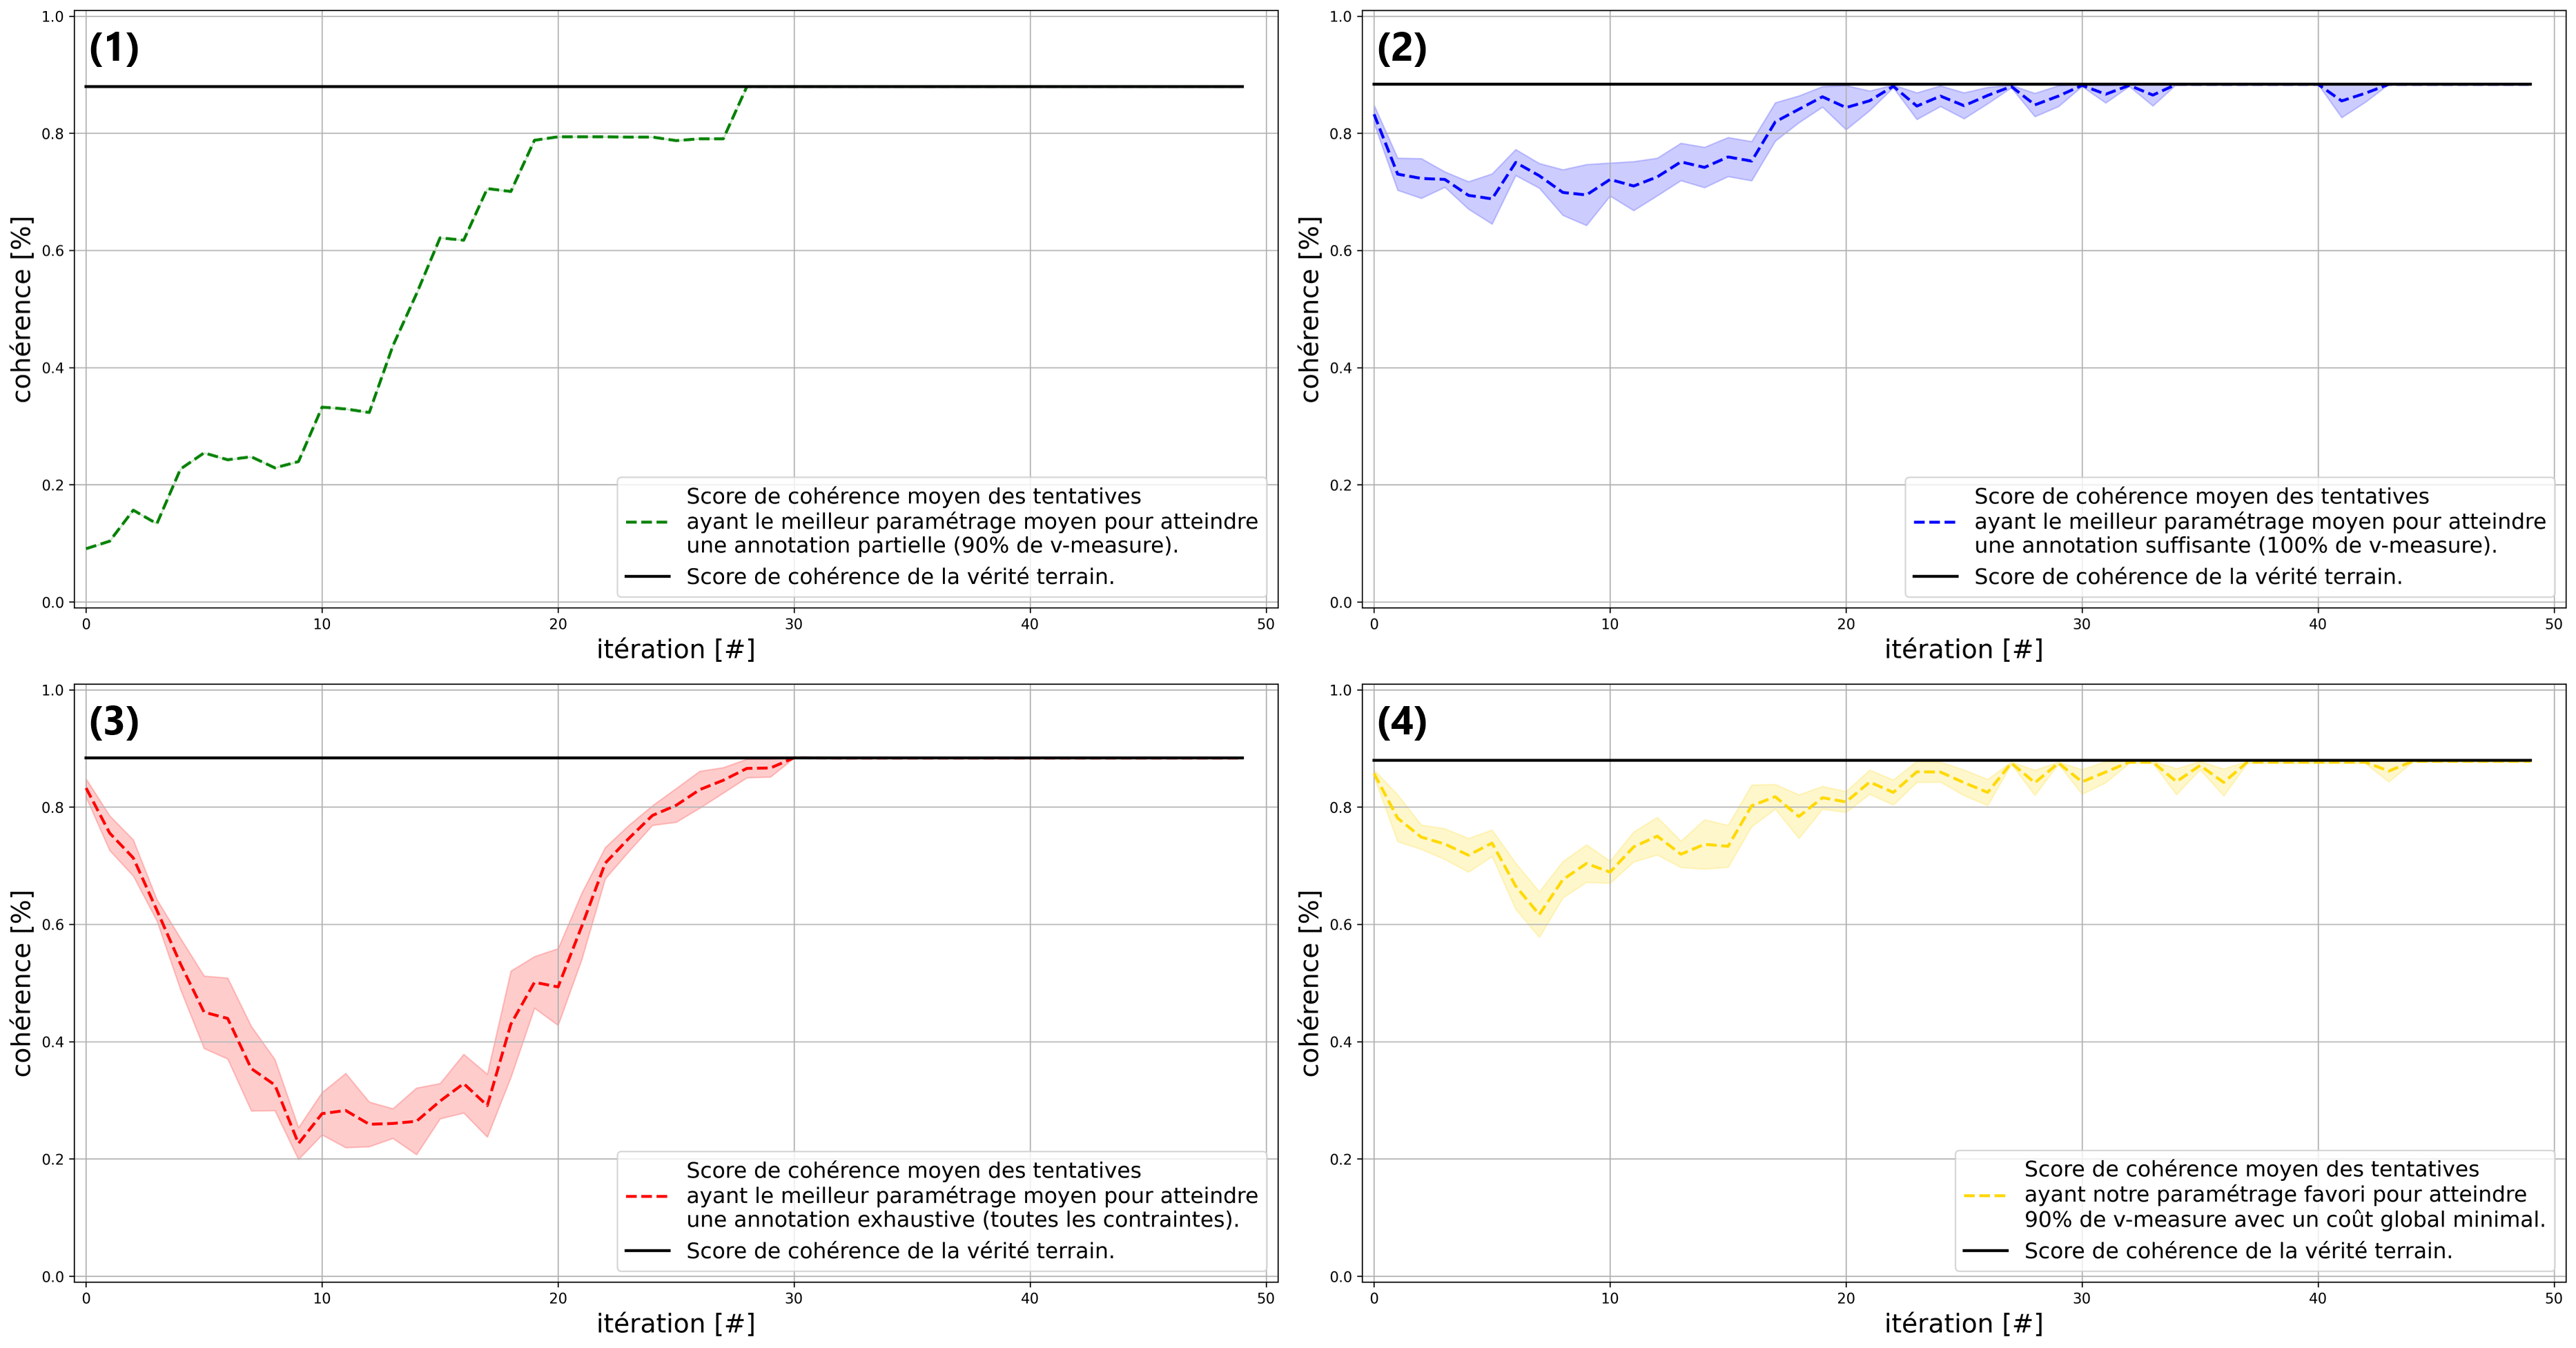
\includegraphics[width=0.95\textwidth]{figures/etude-pertinence-consistence}
	%			\caption{Évolution du score de cohérence moyen des tentatives en fonction de leur paramétrage : \textbf{(1)} meilleur paramétrage moyen une annotation partielle (\texttt{90}\% de \texttt{v-measure}), \textbf{(2)} meilleur paramétrage moyen une annotation suffisante (\texttt{100}\% de \texttt{v-measure}), \textbf{(3)} meilleur paramétrage moyen une annotation exhaustive (annoter toutes les contraintes possibles), et \textbf{(4)} paramétrage favori (\texttt{90}\% de \texttt{v-measure} avec un coût minimal). \\
	%			Note : \textit{Le score de cohérence de la vérité terrain peut varier en fonction des méthodes de prétraitements et de vectorisation utilisées.}}
	%			\label{figure:4.4.4-ETUDE-PERTINENCE-COHERENCE-ANNOTATION}
	%		\end{figure}
	%
	%	%%% Discussion
	%	\subsubsection{Discussion}
	%		\todo[inline]{A REDIGER}
	%	
	%		% Remaques expérience utilisateur.
	%		
	%		% Conclusions et suggestion.